\chapter{Agents}
In this section the different agents are introduced and discussed separately, and in the next section they are compared against each other.
% TODO game concentrate on winning a single round by finishing first and getting points.

\section*{Simplifications}
To limit the scope of the project and to be able to concentrate on the 'card play' aspect of Tichu I decided to simplify the agents as follows:
\begin{description}
    \item[No Trading] The agents all trade random cards. This has the same effect as omitting the trading phase. % TODO This phase is astonishingly complicated to do good and deserves a project for itself. more, influenced by cooperative, tichu, planing, overall strategy
    \item[No Tichu announcement] As mentioned in \ref{sec:tactics}, points won with Tichus often dominate points won by wining tricks. This diverts from the 'card play' aspect, Therefore all Agents are implemented such that they never announce any Tichu % TODO and thus only win by playing better than the opponent. As another consequence, the importance of cooperative play is reduced. % TODO write nicer
    \item[Bombs not anytime] For simplicity and ease of simulation, a player can only play when it's his turn. That means bombs can not be played out of turn. This has not a big impact on the game play overall, since it is rare to gain an advantage in playing a bomb out of turn.
    % TODO  As a result the agents can't learn strategies involving bluffing or 'laying traps' (for example waiting for the Dragon, then bomb it to gain points. or bomb a combination that otherwise can't be beaten.)... would increase branching factor and would slow down mcts considerably. could be made efficient but was too complicated.
    \item[No Wish] For a similar reason as the 'no Tichu' simplification, the agents do not wish any card. % TODO write more
\end{description}

\section{Background}
\label{sec:background}
This section contains a short overview of the main algorithms used by the different agents.

An important notion is the \textbf{gametree}, which is a tree containing as nodes all possible gamestates and as edges the (game)actions leading from a parent state to a child state. The root is the initial state of the game, and the leafs are states in which the game ended (one player or team has won).

\subsection{Minimax Search}
Given a gametree, the optimal strategy can be determined from the minimax value of each node. This value denotes how 'good' a gamestate is for the searching player and is computed as follows:
$$
    minimaxval(s)=
\begin{cases}
    Reward(s), & \text{if s is terminal} \\
    \max_{a\in Actions(s)} minimaxval(next(s, a)), & \text{if player(s) = searching player} \\
    \min_{a\in Actions(s)} minimaxval(next(s, a)), & \text{otherwise}
\end{cases}
$$
where $s$ is a gamestate, $Reward(s)$ denotes the reward for the searching player in $s$, $Actions(s)$ is the set of legal actions in $s$, $player(s)$ denotes the player able to play in $s$ and $next(s, a)$ is the resulting state when playing action $a$ in $s$. \newline
This algorithm performs a complete depth-first search of the gametree, which is computationally unfeasible in most games, but it is a good theoretical baseline for other algorithms.

Despite this, it is possible to use minimax in larger games by stopping at non terminal states and evaluating them with an $utility$ function.
Minimax has been successfully used in games where it is possible to create a good $utility$ function, such as chess.

Furthermore, it is possible to prune away large parts of the searchtree without loosing accuracy using \textbf{alpha-beta pruning}. This method makes use of the fact that some subtrees don't influence the final result since the players never play suboptimal actions. For more details see \cite[chapter 5, p.~170+]{russel14} or any textbook about AI.

\subsection{Monte Carlo Tree Search (MCTS)}
Similar to minimax search, MCTS also searches the gametree, but uses simulated games to evaluate nonterminal states and thus has no need for an utility function. This is especially useful for games where it is hard to determine whether a state is 'good' or 'bad' for a player, for example in games with hidden information, but also in perfect information games such as GO.

The algorithm iteratively builds a subtree of the gametree where the root corresponds to the current state of the game. Each iteration consists of the 4 phases shown in Fig.~\ref{fig:mcts_phases}:
\newline\textbf{Tree Selection} The algorithm traverses the (in previous iterations built up) gametree until it reaches a leaf-node. The decision which actions to follow during the traversal is determined by the \textit{tree policy}. The tree policy attempts to balance considerations of exploration (look in areas that have not been well sampled yet) and exploitation (look in areas which appear to be promising).
An often used tree policy is the UCT (Upper Confidence bound for Trees) formula proposed by \cite{uct} (see section \ref{sec:uct}).
\newline\textbf{Expansion} Once arrived at a leaf state, one more action is chosen and a node for the resulting gamestate is added to the tree. Form this state a \textit{simulation} (or \textit{rollout}) is performed.
\newline\textbf{Simulation} A simulation is the run from a gamestate to a terminal state of the game. During simulation the moves are made according to the \textit{default policy}, which typically chooses an action uniformly at random.
\newline\textbf{Backpropagation} The final state is evaluated and the reward for each player is calculated. The reward is then used to update the statistics of the nodes visited during tree selection, which in turn is used for the \textit{tree policy} in future iterations.

The search can be terminated at any point which makes MCTS especially suitable for games with time or computational resource constraints.

\begin{figure}[h]
    \begin{center}
      \includegraphics[width=0.58\textwidth]{images/basic_mcts_process.png}
      \caption[Basic MCTS process]
      {The basic steps of MCTS. Source \cite{perez13}}
      \label{fig:mcts_phases}
    \end{center}
\end{figure}


\subsection{Determinization and Perfect Information MCTS (PIMCTS)}
\textbf{Determinization} is the process of taking a gamestate with hidden information and creating ('determining') a perfect information state that is consistent with the hidden information. In essence, determinization chooses one out of the many possible perfect information gamestates for a given hidden information gamestate.

To deal with hidden information, PIMCTS performs several instances of MCTS, each on a different determinization. The best action is then chosen based on the results of the individual MCTS.
This approach was successfully used for the game Bridge in \cite{bridge}, but has two main drawbacks, described in \cite{bridge} and further explored in \cite{pimcts} and \cite{ismcts}:
\newline\textbf{Strategy fusion:} An agent can only make one decision in each hidden information state, but in different determinizations different decisions can be made based on the perfect information. This lets the agent 'believe' that he can distinguish between determinizations of the same state, which is not the case. Strategy fusion can cause the agent to choose a bad over a winning action.
\newline\textbf{Nonlocality:} Some determinizations may be vanishingly unlikely (rendering their solutions irrelevant to the overall decision process) due to the other players’ abilities to direct play away from the corresponding states.

\subsection{Information Set MCTS (ISMCTS)}
To tackle the problem of strategy fusion, \textit{Cowling et al.} propose \textit{Information Set MCTS} in \cite{ismcts}. Instead of building a different searchtree for each determinization, ISMCTS builds one search tree with the information from all determinizations using \textit{Information Sets} instead of gamestates as the nodes in the tree. An information set is basically the set containing all indistinguishable gamestates from the the point of view of the player. This allows the sharing of information over different determinizations, which in addition to reducing strategy fusion, provides a basic algorithm with many possibilities for adaptions and improvements. Some of them are implemented in the agents described in the following sections.


\section{Stupid and Random Agent}
To have a baseline, I created the \textit{stupid} and the \textit{random} agent.
The \textit{stupid} agent always passes whenever possible and plays a random single card when passing is not allowed. This is the simplest agent able to play the game, but it is also one of the worst possible agents.

The \textit{random} agent always plays an action chosen uniformly at random from the possible actions.


\section{Minimax Agent}
Even though the gametree for a Tichu game is too big for an exhaustive search I implemented an agent using the minimax algorithm (with alpha-beta pruning).
To complete one search to a depth of 10 (which corresponds not even to one trick) already takes more than a minute (on my machine).
To be able to use it anyway, the agent has the possibility to 'cheat', that is to observe the handcards of the other players, and therefore does not have to search several determinizations.

The simplest $utility$ function for the agent is just \textit{14 - "the number of handcards the player has"} since the goal is to get rid of all cards. However this leads the agent always to play the longest combination possible which turns out not to be a good strategy.
\todo{run minimax vs random}
\todo{when doing experiments with utility of minimax, add them here}

The fact that creating a good $utility$ function needs a lot of \textit{domain knowledge} and that minimax can't deal efficiently enough with the hidden information let me to quickly search for more suitable algorithms.

Side-note: \textit{David Pfander} (\cite{david12}) built an agent for Tichu with a carefully crafted $utility$ function (requiring a lot of \textit{domain knowledge}) and managed to achieve 'average human level' play.


\section{Monte Carlo Tree Search Agents}
MCTS nicely fits the requirements of "using little \textit{domain knowledge}" and is able to deal with hidden information. That makes it an ideal algorithm for this project, and after reading \cite{surveymcts, ismcts, whitehouse14} and their application of ISMCTS on the game \textit{Dou Di Zhu} (which has many similarities to Tichu), I decided to concentrate, for the remainder of the project, on agents using ISMCTS as base algorithm.
In particular on following parts of ISMCTS:
\begin{itemize}
    \vspace{-10px}
    \item Explore possibilities to make better \textit{determinizations} without using \textit{domain knowledge}
    \item Reducing or managing the branching factor
    \item Adding improvements over the ISMCTS and compare them
    \item Finding a better \textit{default policy}(in the simulation phase) than the random strategy
\end{itemize}

In the remainder of this section, I discuss different improvements for the ISMCTS-Tichu agents related to one of the 4 parts. Each of those improvements then is evaluated in the chapter \nameref{ch:experiments}.

\subsection{Default ISMCTS Agent}
The \textit{default ISMCTS agent} builds the basis for the agents improving on the various parts of the algorithm. In this section the \textit{tree policy}, the \textit{state evaluation} and the \textit{selecting of the best action} are determined and used for all other ISMCTS agents, except when stated otherwise.

\subsubsection{Tree selection}
\label{sec:uct}
As hinted at in the \textit{\nameref{sec:background}} section, the simplest and most often used \textit{tree policy} uses the UCT (Upper Confidence bound for Trees) formula proposed by \cite{uct}.
It is derived from viewing the selection problem as a multiarmed bandit problem where each action is an arm and the reward is the result of doing a Monte Carlo simulation after choosing that action.

To be able to use the UCT formula, each node ($n$) keeps track of the number of times it has been visited ($v_n$) and the sum of the rewards the player got after visiting the node ($r_n$).

The \textit{tree policy} is then:
For a given node $p$, select the childnode $c$ that maximizes following formula (ties are broken arbitrarily):
$$
UCT =
\begin{cases}
    \frac{r_c}{v_c} + C\sqrt{\frac{2\ln v_p}{v_c}}, & \text{if } v_c > 0 \\
    FMU, & \text{otherwise} \\
\end{cases}
$$

where $r_c$ is the total reward of the child, $v_p$ is the number of times the current (parent) node has been visited, $v_c$ the number for the child node and $C > 0$ is a constant balancing exploration and exploitation ($\sqrt{2}$ is recommended by \cite{ismcts}). \newline
It is generally recommended that $FMU = \infty$ (First Move Urgency), so that not yet visited child nodes will be visited first before any of them are expanded. However $FMU$ can be set to any value, allowing 'good' children to be expanded before some of their siblings are visited for the first time.

I didn't tune neither $C$ nor $FMU$ and kept them at $\sqrt{2}$ and $\infty$ respectively.


\subsubsection{Evaluation}
\label{sssec:evaluation}
At the end of a rollout, the final state has to be evaluated and the reward is backpropagated trough the gametree. The evaluation thus plays a central role on determining the UCT value of nodes.

I considered following different evaluation strategies (remember that the players from the same team get the same amount of points at the end of a round):
\begin{description}
    \vspace{-10px}
    \item[Absolute Points,] Each team gets the unaltered points as reward.
    \item[Absolute Normalized Points,] The absolute points normalized between -1 and 1
    \item[Relative Points,] Each team gets the difference of points to the other team as the reward. For example, the round ended $70:30$, then the first team gets $70 - 30 = 40$ reward, the second $30 - 70 = -40$ reward.
    \item[Relative Normalized Points,] The relative points normalized between -1 and 1
    \item[Ranking Based,] This evaluation rewards the teams based on the ranking at the end of the round:
        \begin{itemize}
            \vspace{-10px}
            \item $+1$ for a doublewin
            \item $-1$ for a double loss (enemy has doublewin)
            \item $0.5$ for a player of the team finishing first (but no doublewin)
            \item $0$ when an enemy player finished first (but no doublewin)
        \end{itemize}
\end{description}

It turns out that the \textit{ranking based} evaluation produces better results than any of the other strategies (experiments in section~\ref{sec:evaluationexp}). Therefore this evaluation was used for all agents.

\subsubsection{Selecting the best action at the end}
After the search completed, the best action from the initial search-state has to be determined.
The recommended strategy is to select the action corresponding to the most visited node. And indeed that is what I ended up implementing after trying out the two other obvious strategies: taking the node with \textit{highest UCB value} and taking the node with \textit{highest average reward}.

The experiments confirming the recommendation can be found in section~\ref{sec:bestactionexp}.


\subsection{Managing the branching factor}
In \cite{ismcts} it is shown that ISMCTS does not perform significantly better than PIMCTS in \textit{Dou Di Zhu}. However, they suggest this is due to the high branching factor of the game and that in each determinization new possible actions are discovered. Reducing those two factors would increase the advantages of ISMCTS over PIMCTS.

A big reduction of the branching factor comes from the observation that many possible combinations in a given hand are logically identical and thus only one of them has to be considered (see the \textit{\nameref{ch:impl}} section).

Other reductions are achieved by the following two enhancements to ISMCTS.

\subsubsection{Episodic Information Capture and Reuse (EPIC)}

\begin{figure}[h]
\begin{center}
    \subcaptionbox{An example of the \textit{position in epic}. The two circled states have the same \textit{position in epic} but are in a different part of the gametree. Both are reached by action $a$ followed by $b$ from a state where player 2 can play first. However state $AD$ and $AC$ have different \textit{position in epic}. The nodes labeled with $A$ and \textit{P2 first play} also have the same \textit{position in epic}\label{fig:piepic}}%
  [.48\linewidth]{
    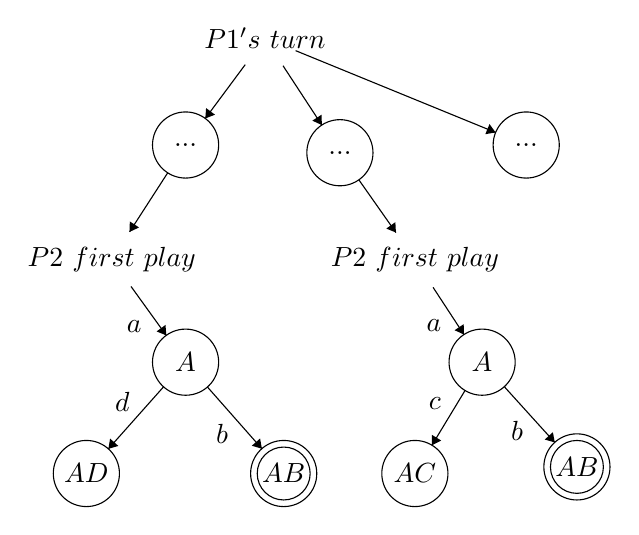
\begin{tikzpicture}[scale=0.14]
        \tikzstyle{every node}+=[inner sep=0pt]
        %\draw [black] (34.6,-5.4) circle (3);
        \draw (34.6,-5.4) node {$P1's\mbox{ }turn$};
        \draw [black] (27.4,-15.1) circle (3);
        \draw (27.4,-15.1) node {$...$};
        \draw [black] (27.4,-34.8) circle (3);
        \draw (27.4,-34.8) node {$A$};
        \draw [black] (41.4,-15.8) circle (3);
        \draw (41.4,-15.8) node {$...$};
        %\draw [black] (20.7,-25.5) circle (3);
        \draw (20.7,-25.5) node {$P2\mbox{ }first\mbox{ }play$};
        %\draw [black] (48.2,-25.5) circle (3);
        \draw (48.2,-25.5) node {$P2\mbox{ }first\mbox{ }play$};
        \draw [black] (54.3,-34.8) circle (3);
        \draw (54.3,-34.8) node {$A$};
        \draw [black] (36.3,-44.9) circle (3);
        \draw (36.3,-44.9) node {$AB$};
        \draw [black] (36.3,-44.9) circle (2.4);
        \draw [black] (62.9,-44.3) circle (3);
        \draw (62.9,-44.3) node {$AB$};
        \draw [black] (62.9,-44.3) circle (2.4);
        \draw [black] (48.2,-44.9) circle (3);
        \draw (48.2,-44.9) node {$AC$};
        \draw [black] (18.4,-44.9) circle (3);
        \draw (18.4,-44.9) node {$AD$};
        \draw [black] (58.3,-15.1) circle (3);
        \draw (58.3,-15.1) node {$...$};
        \draw [black] (32.81,-7.81) -- (29.19,-12.69);
        \fill [black] (29.19,-12.69) -- (30.07,-12.35) -- (29.26,-11.75);
        \draw [black] (25.78,-17.62) -- (22.32,-22.98);
        \fill [black] (22.32,-22.98) -- (23.18,-22.58) -- (22.34,-22.03);
        \draw [black] (22.45,-27.93) -- (25.65,-32.37);
        \fill [black] (25.65,-32.37) -- (25.58,-31.42) -- (24.77,-32.01);
        \draw (23.46,-31.53) node [left] {$a$};
        \draw [black] (36.24,-7.91) -- (39.76,-13.29);
        \fill [black] (39.76,-13.29) -- (39.74,-12.35) -- (38.9,-12.89);
        \draw [black] (43.12,-18.26) -- (46.48,-23.04);
        \fill [black] (46.48,-23.04) -- (46.43,-22.1) -- (45.61,-22.68);
        \draw [black] (49.85,-28.01) -- (52.65,-32.29);
        \fill [black] (52.65,-32.29) -- (52.63,-31.35) -- (51.8,-31.9);
        \draw (50.64,-31.47) node [left] {$a$};
        \draw [black] (29.38,-37.05) -- (34.32,-42.65);
        \fill [black] (34.32,-42.65) -- (34.16,-41.72) -- (33.41,-42.38);
        \draw (31.31,-41.3) node [left] {$b$};
        \draw [black] (56.31,-37.02) -- (60.89,-42.08);
        \fill [black] (60.89,-42.08) -- (60.72,-41.15) -- (59.98,-41.82);
        \draw (58.06,-41.01) node [left] {$b$};
        \draw [black] (52.75,-37.37) -- (49.75,-42.33);
        \fill [black] (49.75,-42.33) -- (50.59,-41.91) -- (49.74,-41.39);
        \draw (50.61,-38.58) node [left] {$c$};
        \draw [black] (25.4,-37.04) -- (20.4,-42.66);
        \fill [black] (20.4,-42.66) -- (21.3,-42.4) -- (20.55,-41.73);
        \draw (22.36,-38.39) node [left] {$d$};
        \draw [black] (37.38,-6.54) -- (55.52,-13.96);
        \fill [black] (55.52,-13.96) -- (54.97,-13.2) -- (54.59,-14.12);
        \end{tikzpicture}
}
~ %add desired spacing between images, e. g. ~, \quad, \qquad, \hfill etc.
  %(or a blank line to force the subfigure onto a new line)
  \subcaptionbox{The EPIC-gamegraph corresponding to the gametree in (a). The two nodes labeled $AB$ are merged as well as the states labeled $A$ and the state where Player 2 can play first.\label{fig:epicgg}}%
[.48\linewidth]{
  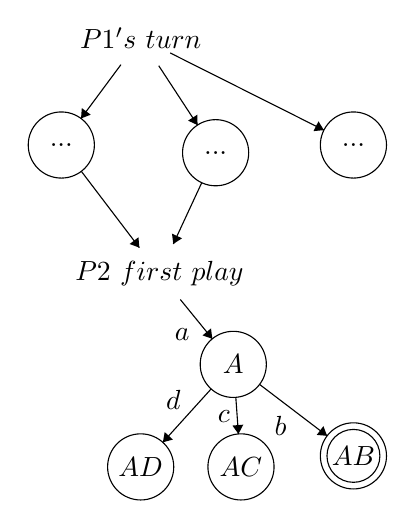
\begin{tikzpicture}[scale=0.14]
    \tikzstyle{every node}+=[inner sep=0pt]
    %\draw [black] (34.6,-5.4) circle (3);
    \draw (34.6,-5.4) node {$P1's\mbox{ }turn$};
    \draw [black] (27.4,-15.1) circle (3);
    \draw (27.4,-15.1) node {$...$};
    \draw [black] (41.4,-15.8) circle (3);
    \draw (41.4,-15.8) node {$...$};
    %\draw [black] (36.3,-26.8) circle (3);
    \draw (36.3,-26.8) node {$P2\mbox{ }first\mbox{ }play$};
    \draw [black] (43,-35) circle (3);
    \draw (43,-35) node {$A$};
    \draw [black] (53.9,-43.3) circle (3);
    \draw (53.9,-43.3) node {$AB$};
    \draw [black] (53.9,-43.3) circle (2.4);
    \draw [black] (43.7,-44.3) circle (3);
    \draw (43.7,-44.3) node {$AC$};
    \draw [black] (34.6,-44.3) circle (3);
    \draw (34.6,-44.3) node {$AD$};
    \draw [black] (53.9,-15.1) circle (3);
    \draw (53.9,-15.1) node {$...$};
    \draw [black] (32.81,-7.81) -- (29.19,-12.69);
    \fill [black] (29.19,-12.69) -- (30.07,-12.35) -- (29.26,-11.75);
    \draw [black] (36.24,-7.91) -- (39.76,-13.29);
    \fill [black] (39.76,-13.29) -- (39.74,-12.35) -- (38.9,-12.89);
    \draw [black] (40.14,-18.52) -- (37.56,-24.08);
    \fill [black] (37.56,-24.08) -- (38.35,-23.56) -- (37.44,-23.14);
    \draw [black] (38.2,-29.12) -- (41.1,-32.68);
    \fill [black] (41.1,-32.68) -- (40.98,-31.74) -- (40.21,-32.37);
    \draw (39.09,-32.33) node [left] {$a$};
    \draw [black] (45.39,-36.82) -- (51.51,-41.48);
    \fill [black] (51.51,-41.48) -- (51.18,-40.6) -- (50.57,-41.4);
    \draw (47.3,-39.65) node [below] {$b$};
    \draw [black] (43.23,-37.99) -- (43.47,-41.31);
    \fill [black] (43.47,-41.31) -- (43.91,-40.47) -- (42.92,-40.55);
    \draw (42.74,-39.7) node [left] {$c$};
    \draw [black] (37.28,-6.75) -- (51.22,-13.75);
    \fill [black] (51.22,-13.75) -- (50.73,-12.95) -- (50.28,-13.84);
    \draw [black] (29.22,-17.49) -- (34.48,-24.41);
    \fill [black] (34.48,-24.41) -- (34.4,-23.47) -- (33.6,-24.08);
    \draw [black] (40.99,-37.23) -- (36.61,-42.07);
    \fill [black] (36.61,-42.07) -- (37.52,-41.82) -- (36.78,-41.14);
    \draw (38.26,-38.19) node [left] {$d$};
    \end{tikzpicture}
    }
  \caption[Epic example]{EPIC example}
  \label{fig:epicex}

\end{center}

\end{figure}

EPIC is an enhancement proposed by \cite{whitehouse14} and aims to take advantage of the episodic nature of certain games. The idea is that instead of discovering the same strategy for very similar situations (episodes) in different parts of the game tree, EPIC puts them together such that those similar situations are the same and thus only have to be discovered once. \newline
It yielded good improvements in \textit{Dou Di Zhu} and it stands to reason that it does also help in Tichu.
\textit{Dou Di Zhu} has the same trick system as Tichu, but it is played with only 3 players and the playable combinations are slightly different. But overall the two games are very close.

In \textit{Dou Di Zhu} and Tichu, an episode is naturally defined by a trick (from first play until all players pass consecutively). The \textit{position in episode} of a node is the path from the node upwards until the beginning of the trick is reached. An example is shown in Fig.~\ref{fig:piepic}
Similar on how all nodes belonging to the same \textit{information set} were put together for ISMCTS, for EPIC, all states with the same \textit{position in epic} are merged into one node creating an EPIC-gamegraph. The result for the example is shown in Fig.~\ref{fig:epicgg}.
For Tichu, the gamegraph contains 4 "root nodes" corresponding to the 4 states where a particular player can play first. \todo{improve example and description}

The search is then performed on this gamegraph according to ISMCTS. To implement EPIC very little change to ISMCT is required. Only the way how gamestates are mapped to nodes has to be modified. The rest of the algorithm is identical.

EPIC reduces the branching factor dramatically since many different nodes are merged. The ordering of different tricks in the game is basically removed, which, of course, introduces some new difficulties and is probably the main reason why it did not perform well on Tichu.

\subsubsection{Move groups}
Another way to reduce the branching factor and possibly improve UCT decisions are \textit{move-grous}.
The idea is to divide the actions into (not necessarily disjoint) groups. Those groups are then inserted as an additional layer after each node in the gametree.
The decision in the \textit{tree policy} then becomes a two-step process. First select a group and then an action belonging to that group (UCT can be used in both phases).
Move groups are introduced in \cite{movegroups} and further examined in \cite{movegroups2}.

This enhancement reduces the effective branching factor and has been shown to help with move selection when similar valued moves appear. However, it is not trivial to find good groups. \cite{movegroups2} found that random groups did neither improve nor worsen the simulation efficiency. Grouping the best nodes together seems to yield the best result, but finding the best nodes is exactly the problem.

The groups I used is to put the actions of the same combination-type into the same group with the idea that they most of the time lead to similar results and thus the chance that the best actions are in the same group are increased.
% TODO NOTE: maybe hight/rank and "probability" are better groups.

Surprisingly, ISMCTS with \textit{move-grous} performed very poorly against the default ISMCTS agent (more in section \ref{sec:movegroupsexp}).


\subsection{Determinization}
\textit{Whitehouse} shows in \cite[p.~54+]{whitehouse14} that for the game \textit{Dou Di Zhu}, more than 20 determinizations per search yield diminishing returns, and the more simulations per determinization are made, the better the agent plays.
Assuming this is value is similar in Tichu I decided to generate 30 different determinizations per search, just to be on the save side (Tichu has one player more).


\subsubsection{Random}
- just randomly assigns the unknown cards to the other players.


\subsubsection{Probabilities}
- Based on some prior probability collected from real game data. - how data is collected
- introduce "General Combinations"
- prior for all nbr handcards (1-14) and for all gencombs: nbr of handcards -> proba of containing general combination.


\subsubsection{Data analysis}
- look at the collected data
- distribution of single cards and pairs are significant different from uniform random


\subsubsection{Pool det}
- a determinization strategy distributing whole combinations on the other players based on 'which combination is most probable to be present and who is most probable to have it'


\subsubsection{Single det}
- looks only at each player in turn and only at single cards.
- "given a player, which cards are most probable to be in his handcards"

\subsubsection{NN det}
- experimental
- tried to learn for each nbr of handcards (N) one model 'given all (unknown) cards, which N cards are most probable to appear'
- did not converge. probably data is too noisy and "near misses" are not counted as correct. There is no concept of 'closeness' of the cards. (ie. giving enemy a 10 instead of a 9 is less 'wrong' than giving a K)



\subsection{Rollout}
\label{sec:rollout}
The rollout phase simulates from a given gamestate to a terminal one following a (fast) action selection strategy. The goal is to estimate an initial value for the state.

\subsubsection{random}
- selects always a random (legal) action.
- Fast but only good when enemy plays randomly.

\subsubsection{Last Good Response With Forgetting (LGRF)}
- still random action selection, but stores all selected action pairs that lead to a win. When encoutering a stored action, then the response (second action in the pair) is chosen instead of random action.
- forgetting is an additional feature, where all stored action responses that lead to a loss are deleted (forgotten).

\subsubsection{no rollout}
- There is the possibility of no rollout. That is all actions are added to the search tree and chosen according to ucb. this is still a random rollowut for states that have never been visited before.

\subsubsection{dqn-nn}
- Instead of choosing the next action randomly, a NN agent (see \ref{sec:nn_agents}) chooses the next action.
- Used in AlphaGo




\section{NN Agents}
\label{sec:nn_agents}
Implementation / Keras-rl
- several network architectures
- several training environments (enemies)


\subsection{Architectures}
- cards as 1-hot encoded vector
- cards grouped by rank vector
- seperate inputs
- current ranking input

\subsection{Training}
- against random
- against former version of itself
- against itself
- against (fast) mcts \\

- policy (Bolzman with variable or fixed tau)

% TODO difficulties?
